%! Tex program = xelatex
\documentclass{article}
%中文
%\usepackage[UTF8]{ctex}
%数学公式
\usepackage{amsmath,amssymb}
%\usepackage{ntheorem}
%\usepackage{mdframed} %公式框1
% e.g., \newmdtheoremenv{theorem}{Theorem}
\usepackage{amsthm}
%边界
\usepackage[letterpaper,top=1cm,bottom=2cm,left=3cm,right=3cm,marginparwidth=1.75cm]{geometry}%table package
%Table
\usepackage{multirow,booktabs}
\usepackage{makecell}
%字体颜色
\usepackage{color}
\usepackage[dvipsnames]{xcolor}  % 更全的色系
%代码
\usepackage[OT1]{fontenc}
% MATLAB 代码风格
\usepackage[framed,numbered,autolinebreaks,useliterate]{/Users/anye_zhenhaoyu/Desktop/Latex/mcode}
\usepackage{listings}
\usepackage{algorithm}
\usepackage{algorithmic}
\usepackage{pythonhighlight} % Python
%插图
\usepackage{graphicx}
%改变item格式
\usepackage{enumerate}
%物理
\usepackage{physics}
%extra arrows
\usepackage{extarrows}
% caption(居中指令)
%\usepackage[justification=centering]{caption}
\usepackage{caption}
% htpb
\usepackage{stfloats}
% pdf 拼接
\usepackage{pdfpages}
% 超链接url
\usepackage{url}

\def\RR{\mathbb{R}}
\def\ZZ{\mathbb{Z}}
\def\EE{\mathbb{E}}

\def\Trsp#1{#1^{\mathcal{T}}}
\def\LT{\mathcal{L}}

\def\bold#1{\boldsymbol{#1}}
\def\bw{\boldsymbol{\omega}}
\def\ba{\boldsymbol{a}}
\def\bb{\boldsymbol{b}}
\def\bc{\boldsymbol{c}}
\def\bd{\boldsymbol{d}}
\def\be{\boldsymbol{e}}
\def\bf{\boldsymbol{f}}
\def\bg{\boldsymbol{g}}
\def\bh{\boldsymbol{h}}
\def\bt{\boldsymbol{t}}
\def\bu{\boldsymbol{u}}
\def\bv{\boldsymbol{v}}
\def\bx{\boldsymbol{x}}
\def\by{\boldsymbol{y}}
\def\bz{\boldsymbol{z}}

\def\bA{\boldsymbol{A}}
\def\bB{\boldsymbol{B}}
\def\bC{\boldsymbol{C}}
\def\bE{\boldsymbol{E}}
\def\bF{\boldsymbol{F}}
\def\bG{\boldsymbol{G}}
\def\bL{\boldsymbol{L}}
\def\bM{\boldsymbol{M}}
\def\bO{\boldsymbol{O}}
\def\bP{\boldsymbol{P}}
\def\bQ{\boldsymbol{Q}}
\def\bX{\boldsymbol{X}}
\def\bY{\boldsymbol{Y}}

\def\Esolve{\textcolor{blue}{Solve: }}
\def\Eproof{\textcolor{blue}{Proof: }}
\def\case#1{\textcolor{blue}{Case \uppercase\expandafter{\romannumeral#1}: }}

\def\suminf#1{\sum_{#1=-\infty}^{+\infty}}

\newtheorem{lemma}{Lemma}
\newtheorem{theorem}{Theorem}
\newtheorem{defination}{Definition} 

\graphicspath{{figures/}}

\begin{document}
\title{Homework 13}
\author{Zhen}
\maketitle

\section*{Problem 1}
\begin{enumerate}[(a)]
	\item 
		By the fact that $f(x)$ is monotone increasing, the optimal solution is $x=0$ and the optimal value $f^*$ is $\log 2$.
	\item
		The dual function is
		\[
		    \begin{aligned}
				\phi(\mu)
				&=
				\inf_x\qty[f(x)-\mu x]
				=
				\inf_x\qty[\log\frac{1+e^x}{e^{\mu x}}]
				=
				\log\qty[\inf_{t>0}\qty(\frac{1+t}{t^\mu})]
				\\[5pt]&=
				\begin{cases}
					-\infty &\qif\mu>1
					\\
					-(1-\mu)\log(1-\mu)-\mu\log\mu
					&\qif0\le\mu\le1
					\\
					-\infty&\qif\mu<0
				\end{cases}
		    \end{aligned}
		\]
		The dual problem is
		\[
		    \begin{aligned}
		        \max_\mu\ \ \ &\phi(x)=
				\begin{cases}
					-(1-\mu)\log(1-\mu)-\mu\log\mu
					&\qif0\le\mu\le1
					\\
					-\infty&\qotherwise
				\end{cases}
				\\
				\qq*{s.t.}&\mu\ge0
		    \end{aligned}
		\]
	\item
		\[
		    \begin{aligned}
				\phi'(\mu)=\log\qty(\frac{1-\mu}{\mu})
		    \end{aligned}
		\]
		Thus the dual optimal solution is $\mu=\flatfrac{1}{2}$ and $\phi^*=\log 2$. The strong duality holds.
\end{enumerate}


\section*{Problem 2}
\begin{enumerate}[(a)]
    \item
		The Lagrange dual function is
        \[
            \begin{aligned}
				\phi(\mu_1,\mu_2)&=
				\inf_x\qty[
					(\mu_1+\mu_2+1)x_1^2
					-2(\mu_1+\mu_2)x_1
					+(\mu_1+\mu_2+1)x_2^2
					-2(\mu_1-\mu_2)x_2
					+\mu_1+\mu_2
				]
				\\[5pt]&=
				\begin{cases}
					\mu_1+\mu_2
					-2\flatfrac
					{(\mu_1^2+\mu_2^2)}{(\mu_1+\mu_2+1)}
					&\qif \mu_1+\mu_2+1\ge0
					\\
					-\infty &\qif \mu_1+\mu_2+1<0
				\end{cases}
            \end{aligned}
        \]
		Thus the dual problem is
		\[
			\begin{aligned}
				\max_{\mu_1,\mu_2}\ \ \ &
				\phi(\mu_1,\mu_2)=
				\begin{cases}
					\mu_1+\mu_2
					-2\flatfrac
					{(\mu_1^2+\mu_2^2)}{(\mu_1+\mu_2+1)}
					&\qif \mu_1+\mu_2+1\ge0
					\\
					-\infty &\qif \mu_1+\mu_2+1<0
				\end{cases}
				\\
				\qq*{s.t.} &\mu_1,\mu_2\ge 0
			\end{aligned}
		\] 
    \item
		\[
			\phi(\mu_1,\mu_2)
			=-\frac{(\mu_1-\mu_2)^2}{\mu_1+\mu_2+1}+
			\frac{\mu_1+\mu_2}{\mu_1+\mu_2+1}
			\le
			\frac{\mu_1+\mu_2}{\mu_1+\mu_2+1}
		\]
		Thus $\phi^*=1$. The strong duality holds.
	\item
		Slater’s condition does not hold (no point in $\mbox{int} D$ is feasible). Thus Slater’s condition is not the necessary condition for strong duality.
	\item
		$\phi(\mu_1,\mu_2)=\phi^*\iff\mu_1=\mu_2\to+\infty$.
		The dual optimal value $\phi^*$ is not attained by any dual feasible point.
		This is expected because $\bx^*$ is not regular.
\end{enumerate}

\section*{Problem 3}
\begin{enumerate}[(a)]
    \item
		\[
		    \begin{aligned}
				\phi(\mu)
				&=
				\inf_{x_1,x_2\ge0}
				\qty[x_1^3+x_2^3+\mu(1-x_1-x_2)]
				\\&=
				\begin{cases}
				    \mu
					-\frac{4}{3\sqrt{3}}\mu^{\flatfrac{3}{2}}
					&\qif\mu\ge0
					\\
					\mu&\qif\mu<0
				\end{cases}
		    \end{aligned}
		\]
    \item
		$\phi(\mu)$ reaches the maximum at the point $\mu=\flatfrac{3}{4}$. Thus the dual optimal value is $\phi^*=\frac{1}{4}$.
	\item
		We only need to consider the cases where $x_1,x_2\ge 0$.
		\[
			f(\bx)=x_1^3+x_2^3
			\ge
			2(\frac{x_1+x_2}{2})^3
			\ge \frac{1}{4}
		\]
		Finally, $f(\flatfrac{1}{2},\flatfrac{1}{2})=\flatfrac{1}{4}=f^*$
	\item
		The dual function is
		\[
		    \begin{aligned}
		        \phi(\mu_1,\mu_2,\mu_3)
				&=
				\inf_{x_1,x_2}\qty[
					x_1^3+x_2^3+\mu_1(1-x_1-x_2)
					-\mu_2x_1-\mu_3x_2
				]
				=-\infty
		    \end{aligned}
		\]
		Strong duality does not hold for (P2).
\end{enumerate}

\section*{Problem 4}

\begin{enumerate}[(a)]
    \item
		By Slater's condition, $f(\bw^*,b^*)=f^*=\phi^*=\phi(\bold{\mu}^*)$. By KKT condition, if $\mu_i\neq0$, then $1-y_i(\bx_i^T\bw+b)=0$. 

		Thus we have $b^*=y_i-\bx_i^T\bw^*$ ($y_i^2=1)$.
    \item
		The output is\\
		\texttt{
			primal optimal:\\
			w = [-1.09090895  1.45454542]\\
			b = -0.09090925328321615
			\\
			\\
			dual optimal:\\
			mu = [1.65289246e+00 -0.00000000e+00 -0.00000000e+00 -0.00000000e+00\\
 -0.00000000e+00 -0.00000000e+00 -0.00000000e+00  1.65289239e+00\\
 -0.00000000e+00 -0.00000000e+00  7.15316505e-08 -0.00000000e+00\\
 -0.00000000e+00]
		}
		\begin{figure}[H]
			\centering
			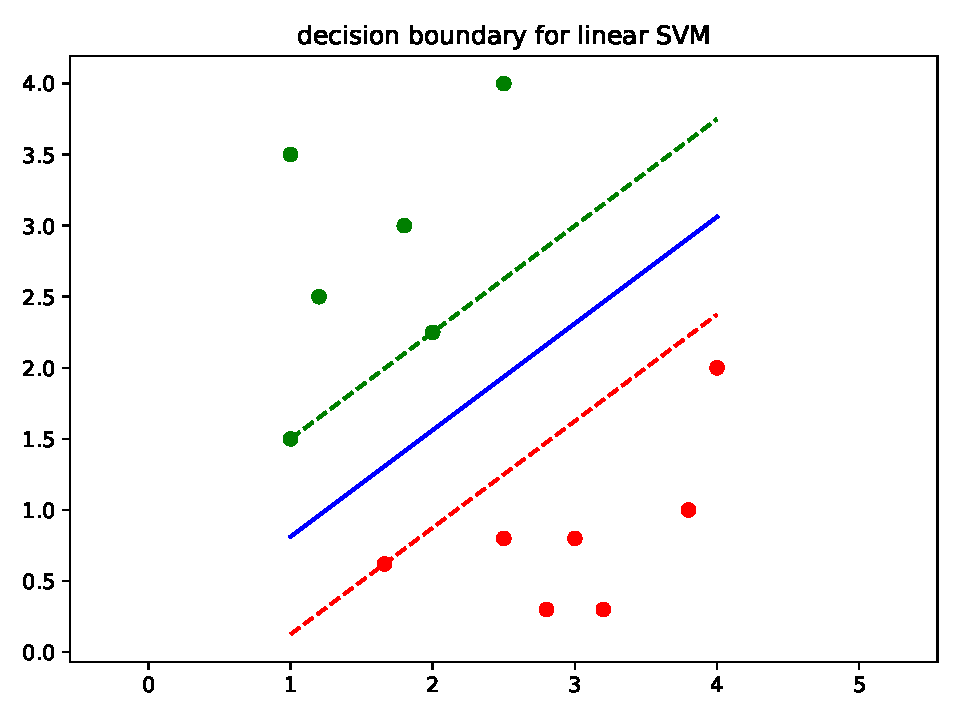
\includegraphics[width=0.8\linewidth]{svm.pdf}
		\end{figure}
\end{enumerate}

\end{document}

